\documentclass[a4paper,12pt]{article}

\usepackage{wrapfig}
\usepackage{graphicx}
\usepackage{mathtext}
\usepackage{amsmath}
\usepackage{siunitx} % Required for alignment
\usepackage{multirow}
\usepackage{rotating}
\usepackage{float}
\usepackage{booktabs}
\usepackage{color, colortbl}

\usepackage[russian]{babel}

%Light gray:
\definecolor{Gray}{gray}{0.9}

\graphicspath{{pictures/}}

\title{\begin{center}Лабораторная работа №1.1.1\end{center}
Определение удельного сопротивления нихромовой проволки}
\author{Мыздриков Иван}
\date{\ 5 сентября 2024 г.}


\begin{document}
    \pagenumbering{gobble}
    \maketitle
    \newpage
    \pagenumbering{arabic}

    \section{Введение}
    \textbf{Цель работы:}
    \begin{itemize}
        \item измерить удельное сопротивление нихромовой проволки двумя способами
        \item вычислить систематические и случайные ошибки
    \end{itemize}

    \vspace{1cm}

    \textbf{В работе используются: }
    \begin{itemize}
        \item линейка
        \item штангенциркуль
        \item микрометр
        \item отрезок проволки из нихрома
        \item амперметр
        \item вольтметр
        \item мост постоянного тока
    \end{itemize}

    \newpage
    \section{Ход работы}
    \paragraph{}
    Для расчета удельного сопротивления измерим сопротивление проволки с известной геометрией и высчитаем удельное сопротивление по формуле
    \begin{equation}
        \rho = \frac{R}{l}\frac{\pi d^{2}}{4}\
    \end{equation}
    где $R$ - сопротивление проволки, $l$ -длина проволки, $d$ - диаметр проволки.

    \paragraph{}
    Измерения мы буедм проводить для 3х длин проволки - $50, 30, 20$ $см$.
    \paragraph{}
    Для начала измерим толщину проволки, учитывая что из за неровностей она меняется по длине проволки, поэтому измерим его в нескольких точках и усредним.
    При измерении штангенциркулем везде получаем одно и то же значение

    \[d_{шц} = (0.35 \pm 0.05) мм\]

    \vspace{0.5cm}

    \begin{center}
        При измерении микрометром получаем значения
    \end{center}

    \begin{table}[H]
        \begin{center}

         \begin{tabular}{|c|c|c|c|c|c|c|c|c|c|c|}
            \hline
            \multirow{1}{*}{\textbf{$d, мм$}}
            & 0.36 & 0.36 & 0.35 & 0.35 & 0.36 & 0.34 & 0.35 & 0.36 & 0.35 & 0.36\\
            \hline
        \end{tabular}
            \caption{Измерения диаметра проволки микрометром}
        \end{center}

    \end{table}
    \paragraph{}
    Усреднив значения из таблицы, посчитав дисперсию выборки и суммировав её с систематической ошибкой $\Delta d_{сист} = 0.005мм$ получаем

    \[d_{мр} = (0.354 \pm 0.005)мм\]

    \paragraph{}
    Сразу же подсчитаем площадь поперечного сечения для обоих случаев

    \begin{align*}
        S_{мр} &= (0.098 \pm 0.003)мм^2
    \end{align*}

    \newpage

    \begin{table}[H]
        \begin{center}

        \begin{tabular}{|l|r|r|r|r|r|r|}
        \hline
        $l, см$ & \multicolumn{2}{c|}{20} & \multicolumn{2}{c|}{30} & \multicolumn{2}{c|}{50} \\
        \hline
        {№} &      $U, мВ$ &        $I, мА$&      $U, мВ$ &         $I, мА$ &    $U, мВ$ &         $I, мА$ \\
        \hline \rowcolor{Gray}
        1  &  505 & 273 & 640 & 211 &  655 & 130 \\
        2  &  360 & 178 & 450 & 150 &  585 & 117 \\\rowcolor{Gray}
        3  &  310 & 152 & 350 & 115 &  515 & 108 \\
        4  &  240 & 116 & 290 &  96 &  425 &  84 \\\rowcolor{Gray}
        5  &  180 &  89 & 235 &  77 &  385 &  77 \\
        6  &  145 &  70 & 195 &  64 &  335 &  67 \\

        \hline
        \end{tabular}
            \caption{Измерении зависимости $U(I)$ при различных $l$}
        \end{center}

    \end{table}

    \paragraph{}

    \begin{wrapfigure}{l}{0.5\linewidth}
        \begin{center}
            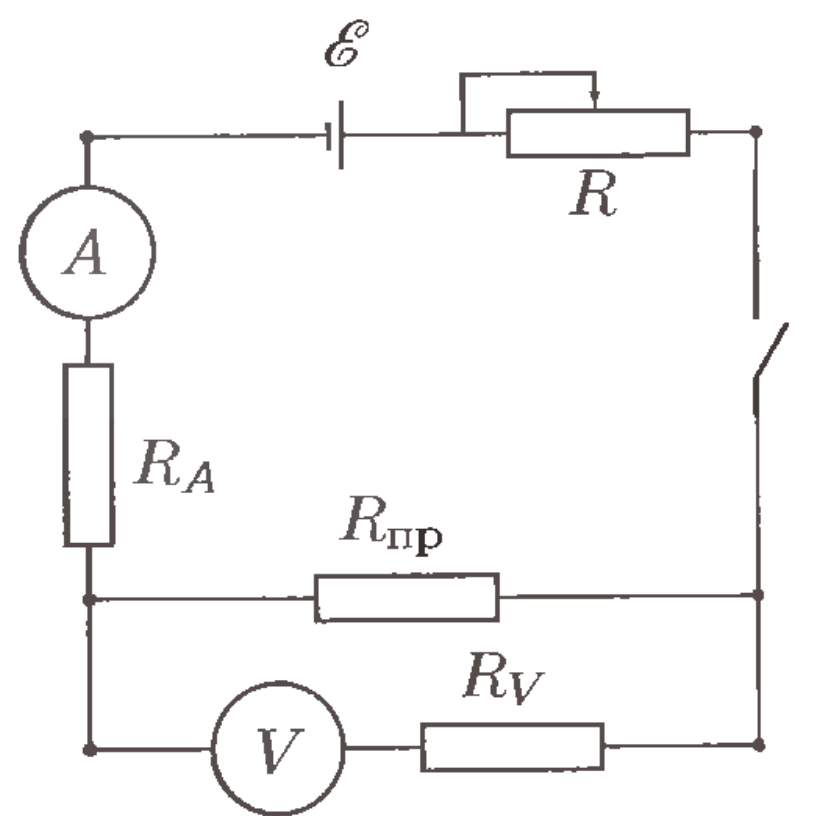
\includegraphics[scale=0.3]{sxema.png}
            \caption{Схема установки}
        \end{center}
    \end{wrapfigure}
    Измерения будем проводить по схеме ниже. Обозначим показания вольтметра как $U$, а амперметра как $I$. Легко получить формулу для $R_{пр}$
    \[R_{пр} = \frac{U}{I}\left(1 + \frac{U/I}{R_{v}}\right)\]
    \paragraph{}
    Из чарактеристик вольтметра знаем что сопротивление вольтметра порядка 4.095$k\Omega$, поэтому поправка $\frac{U/I}{R_v}$  $0.5\%$, что больше относительных погрешностей вольтметра и амперметра в $2.5$ раза. Исходя из этого пренебрежем влиянием сопротивления вольтметра и воспользуемся приближенной формулой
    \[R_{пр}\approx\frac{U}{I}\]
    \newpage
    \paragraph{}
    Для нахождения сопротивления построим график $U(I)$, и из наклона прямой найдем сопротивление. Из графика получаем следующие данные.
   
    \begin{table}[H]
        \begin{center}

            \begin{tabular}{|l|r|r|r|}
            \hline
            $l, см$          &  20 & 30 & 50 \\
            \hline
            $R_{пр}, \Omega$ &  $1.787\pm0.14$ & $3.018\pm0.041$  & $4.425\pm0.85$\\
            \hline
            \end{tabular}
            \caption{Расчетные $R_{пр}$ от $l$}
        \end{center}

    \end{table}
    \paragraph{}
    Сравним с данными измерении от моста Р4833.

    \begin{table}[H]
        \begin{center}

        \begin{tabular}{|l|r|r|r|}
        \hline
        $l, см$          &  20 & 30 & 50 \\
        \hline
        $R_{пр}, \Omega$ &  $2.057\pm0.01$ & $3.046\pm0.01$ & $5.059\pm0.01$ \\
        \hline
        \end{tabular}
            \caption{$R_{пр}$ от $l$ по измерениям Р4833}
        \end{center}

    \end{table}

    \paragraph{}
    Рассмотрим на сколько процентов расчетные сопротивления меньше имерянных.

    \begin{table}[H]
        \begin{center}

        \begin{tabular}{|l|r|r|r|}
        \hline
        $l, см$          &  20 & 30 & 50 \\
        \hline
        $\varepsilon, \%$ &  13.1 & 0.075 & 12.53 \\
        \hline
        \end{tabular}
            \caption{Различие между сопротивлениями}
        \end{center}

    \end{table}

    \paragraph{}
    Эти различия очень большие и никак не объясняются погрешностями. Так как график идеально линейный только при $l$=30см и совпадает со значениями моста при этом же условии, стоит предположить, что в измерениях вольтметра и амперметра была дополнительная ошибка при  $l$=20см и  $l$=50см. Вероятно она вызвана человеческим фактором (неправильное округление при записи измерений), потому стоит использовать значения моста для измерения удельного сопротивления.    
    \paragraph{}
    Погрешность моста в диопазоне измерении $\pm0.01\Omega$.
    Воспользуемся формулами для подсчета удельного сопротивления и его погрешности.

    \begin{align*}
        \rho &= \frac{RS}{l}\\
        \Delta\rho &= \rho\sqrt{\left(\frac{\Delta R}{R}\right)^2 + \left(\frac{\Delta S}{S}\right)^2 + \left(\frac{\Delta l}{l}\right)^2}
    \end{align*}
    \paragraph{}
    Для площади сечения $S$ воспользуемся значением, полученным с помощью микрометра. Подставляя числа получаем


    \begin{table}[H]
        \begin{center}

        \begin{tabular}{|l|r|r|r|}
        \hline
        $l, см$          &  20 & 30 & 50 \\
        \hline
        $\rho, \Omegaм$ &  10.08 & 9.95 & 9.91 \\
        \hline
        $\Delta\rho, \Omegaм$ &  0.31 & 0.3 & 0.3 \\
        \hline
        \end{tabular}
            \caption{Различие между сопротивлениями при использовании моста}
        \end{center}

    \end{table}

    \begin{table}[H]
        \begin{center}

        \begin{tabular}{|l|r|r|r|}
        \hline
        $l, см$          &  20 & 30 & 50 \\
        \hline
        $\rho, \Omegaм$ & 8.756 & 9.98 & 8.673\\
        \hline
        $\Delta\rho, \Omegaм$ & 8.41 & 0.33 & 1.94 \\
        \hline
        \end{tabular}
            \caption{Различие между сопротивлениями при первом способе (вольтметр и амперметр)}
        \end{center}

    \end{table}

    Как ответ запишем среднее  \[\rho = (9.98 + 0.31)\Omegaсм, \varepsilon_{\rho} \approx 3\%\]

    \section{Заключение}
    Значение удельного сопротивления совпадает с табличными значениями для нихрома. Значении сопротивлении измерянных косвенным методои оказались в среднем на $5\%$ ниже реальных, что скорее всего объясненяется либо некалиброванностью вольтметра, либо его аномальной малостью внутреннего сопротивления вольтметра (порядка $100\Omega$). В любом случае даже использовав заниженные сопротивления приходим к тому же выводу что проволка действительно нихромовая.
    \newpage



    \begin{sidewaysfigure}
        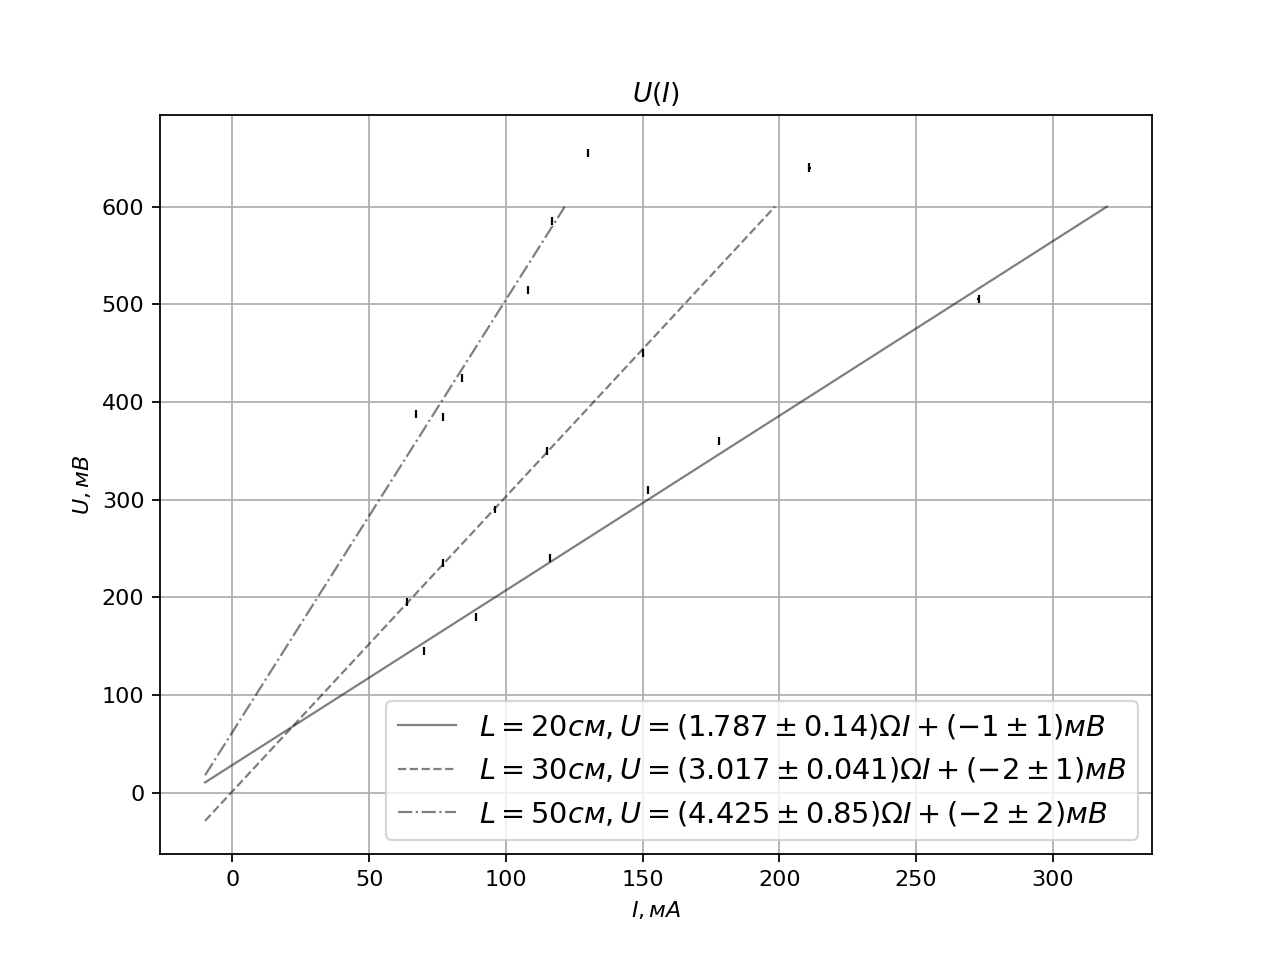
\includegraphics[scale=1]{grafik.png}
        \caption{График зависимости $U(I)$}
    \end{sidewaysfigure}
\end{document}
